 \documentclass[final]{beamer}
 \usetheme{Berlin} 
 %\usecolortheme{beaver}


%%%%lualatex on
%\usepackage{luatextra}
\usepackage{fontspec}
\usepackage{amsmath}
%Ligatures={Contextual, Common, Historical, Rare, Discretionary}
%\setmainfont[Mapping=tex-text]{Linux Libertine O}

\usepackage{natbib}
\usepackage{mathptmx}
\usepackage{latexsym}
\usepackage{mathtools}
%\usepackage[colorgrid,texcoord]{eso-pic}
\usepackage[absolute,overlay]{textpos}

\usepackage[orientation=landscape, size=a0, scale=1.4]{beamerposter}



\DeclarePairedDelimiter\abs{\lvert}{\rvert}%
\DeclarePairedDelimiter\norm{\lVert}{\rVert}%


\makeatletter
\let\oldabs\abs
\def\abs{\@ifstar{\oldabs}{\oldabs*}}
\let\oldnorm\norm
\def\norm{\@ifstar{\oldnorm}{\oldnorm*}}
\makeatother

\title{
	Agent Based Modelling  \& History
}

\date{Granada, ICSS , 2015}
\author{Simon Carrignon$^1$}
\institute[]{
	$^1$Barcelona~Supercomputing~Center \\

}

\begin{document}
\begin{frame}
	\maketitle
	\begin{columns}
		\column{0.33\textwidth}
		\begin{block}{Introduction}
			Understand the economics of our society is a complex task as it involve interaction between complex social structures. But understand past economics is another problem as in that case researcher cannot observe directly the phenomenon they want to understand but can only infer it using byproduct of this process that have remains somehow through the move of age. Using those remaining artefact historien and archaeologists proposed hypothesis about the process at the roigine of such byproduct. Often those hypothesis are sentences that are difficult to compare. We propose that embedded those hypothese into Agent Based Modelisation would allow to better test such hypothesis while allowing to better taking into account of historical context.
		\end{block}
		\column{0.33\textwidth}
		\column{0.33\textwidth}

		\begin{block}{WEUBI}
			Understand the economics of our society is a complex task as it involve interaction between complex social structures. But understand past economics is another problem as in that case researcher cannot observe directly the phenomenon they want to understand but can only infer it using byproduct of this process that have remains somehow through the move of age. Using those remaining artefact historien and archaeologists proposed hypothesis about the process at the roigine of such byproduct. Often those hypothesis are sentences that are difficult to compare. We propose that embedded those hypothese into Agent Based Modelisation would allow to better test such hypothesis while allowing to better taking into account of historical context.
		\end{block}
	\end{columns}
	\begin{columns}
		\column{0.33\textwidth}
	\begin{block}
		{Monte Testaccio}

		An amphora garbage in Roma.\\

		\begin{center}
			\includegraphics[height=3cm]{./Mount-Testaccio.jpg}
			\hfil \includegraphics[height=3cm]{./Mount-Testaccio2.jpg}\\
			\vfill
			\includegraphics[height=3cm]{./titulus.png}

		\end{center}


		About 47000 amphora from CEIPAC database and other data in other databases (places in Pleiade, Greek names in Oxford...)

		\begin{center}
			\includegraphics[width=9cm]{./fortGreekPlaceAndAmphora.png}
		\end{center}
	\end{block}

		\column{0.33\textwidth}
	\begin{block}{Roman Economy}
		\begin{center}
			\Huge
			What was the nature of the Roman Economy?\\
		\end{center}

		\vfill

		\begin{block}
			{The primitivism/modern debate}
			The Roman Economy was already a free-market similar as today vs all price were fixed by the state, no free market, us of slave.
		\end{block}
	\end{block}
		\column{0.33\textwidth}

	\begin{block}{Computer Model}

		An Agent Based Model mixing to main aspects (WSC -- 2015):

		\vfil
		\begin{enumerate}
			\item a	simple bargain mechanism,
			\item and (cultural) evolutionary dynamics.
		\end{enumerate}

		\vfill
		$\rightarrow$ Implement a ``simple'' theoretical abstract model, \emph{to be ``complexified''}.




		\begin{block}{Bargaining}
			\begin{itemize}
				\item Agents have :
					\begin{itemize}
						\item Goods
						\item Value they attribute to goods
					\end{itemize}
				\item Agents produce 1 good and use it to exchange for the other goods, given the value they associate to each good.
				\item After the exchange, agents consume the goods and get a ``score'' (utility?) depending on the amount of good they gather and a scale of ``universal intrinsic value'' for each good.
			\end{itemize}

		\end{block}

		\begin{block}{Evolving}
			After 10 steps of exchange :
			\begin{itemize}
				\item  The less successful (in term of utility) agents copy the set of value of the most successful agent (Biased-Copy/selection).
				\item Given a probability $\mu$ the value attributed to some goods are modified (Innovation/Mutation)
			\end{itemize}

		\end{block}

%	\begin{center}
%		\includegraphics[width=1.5\textwidth]{simsoc-stage1-small}
%	\end{center}


		Illustrate the opacity :
		\begin{itemize}
			\item 	\alert{One simulation : 57min}
			\item	100 simulations (statistical need) : 5700min $\approx$ 4 days
		\end{itemize}

		Lets try with :
		\begin{itemize}
			\item 	10 different probability exchange right. (0.001 to 0.20)
			\item 	3 size of population (250 , 500 , 1000)
			\item 	And different number of goods : (3, 6 , 9)
		\end{itemize}

		\begin{center}
			$= 10 \times 3 \times 3 = 90 $ ``environments'' (experimental setups).\\
			\vfill
			$\rightarrow$ \alert{360 days of continuous simulations.}


		\end{center}



	\end{block}
	\end{columns}


	\begin{columns}
		\column{0.33\textwidth}
		\begin{block}{Price Equilibrium}

			\begin{block}{Result for 3 goods and 500 agents}
				Without surprise, the system evolves toward an equilibrium where all agents adopt optimal prices (clearing-market prices). 
			\end{block}
			\begin{columns}
				\column{5cm}
				\includegraphics[height=2cm]{./ClearingPriceDistanceEvolutionForTrade-G3N500.pdf}
				\column{35cm}
				\includegraphics[width=2cm]{./scoreEx1.png}\\
				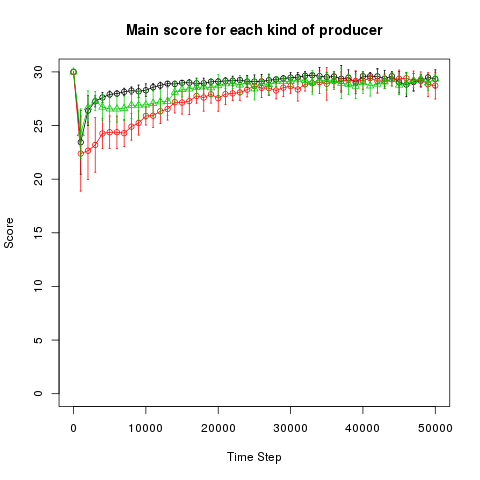
\includegraphics[width=2cm]{./scoreEx2.png}
			\end{columns}

		\end{block}



		\column{0.33\textwidth}
		\begin{block}{Price Equilibrium}
			\begin{center}
				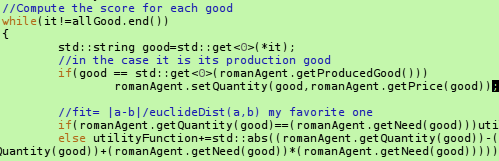
\includegraphics[width=1cm]{./codePrices.png}\\
			\end{center}

			\begin{center}

				\includegraphics[width=1cm]{./codeNeeds.png}\\
			\end{center}
			\begin{center}

				\includegraphics[width=1cm]{./codeNeeds.png}\\
				\includegraphics[width=5cm]{./NonEquilibrium.png}
			\end{center}


		\end{block}

		\column{0.33\textwidth}
		\begin{block}{Price Equilibrium}
			\begin{columns}
				\column{.5\textwidth}
				\includegraphics[height=5cm]{./NonEquilibrium.png}
				\column{.35\textwidth}
				\includegraphics[width=\textwidth]{./scoreEx1b.png}\\
				\includegraphics[width=\textwidth]{./scoreEx2b.png}
			\end{columns}


		\end{block}
	\end{columns}
			What does all that mean?\\

			Epistemological uncertainty\dots
			\vfill
			\begin{center}
				\Huge
				What was the nature of the Roman Economy?\\
			\end{center}
			\vfill

			De-idealization needed, yes, but how?
			\begin{itemize}
				\item A ``guided'' de-idealization? 
			\end{itemize}


			\begin{center}
				Thanks for you attention.\\
				\vfil

				\includegraphics[width=2cm]{./bsc.jpeg}
			\end{center}


	\begin{equation}\label{eq:score}
		s^i_j = \begin{cases}
			s_{max}=1 & \text{if $q^i_j = n_j$}\\
			1 -\dfrac{\abs{q^i_j - n_j}}{ \sqrt{\abs{(q^i_j)^2-(n_j)^2}}} & \text{if $q^i_j \neq   n_j$}
		\end{cases}
	\end{equation}


	\begin{figure}[htp]
		\begin{center}
			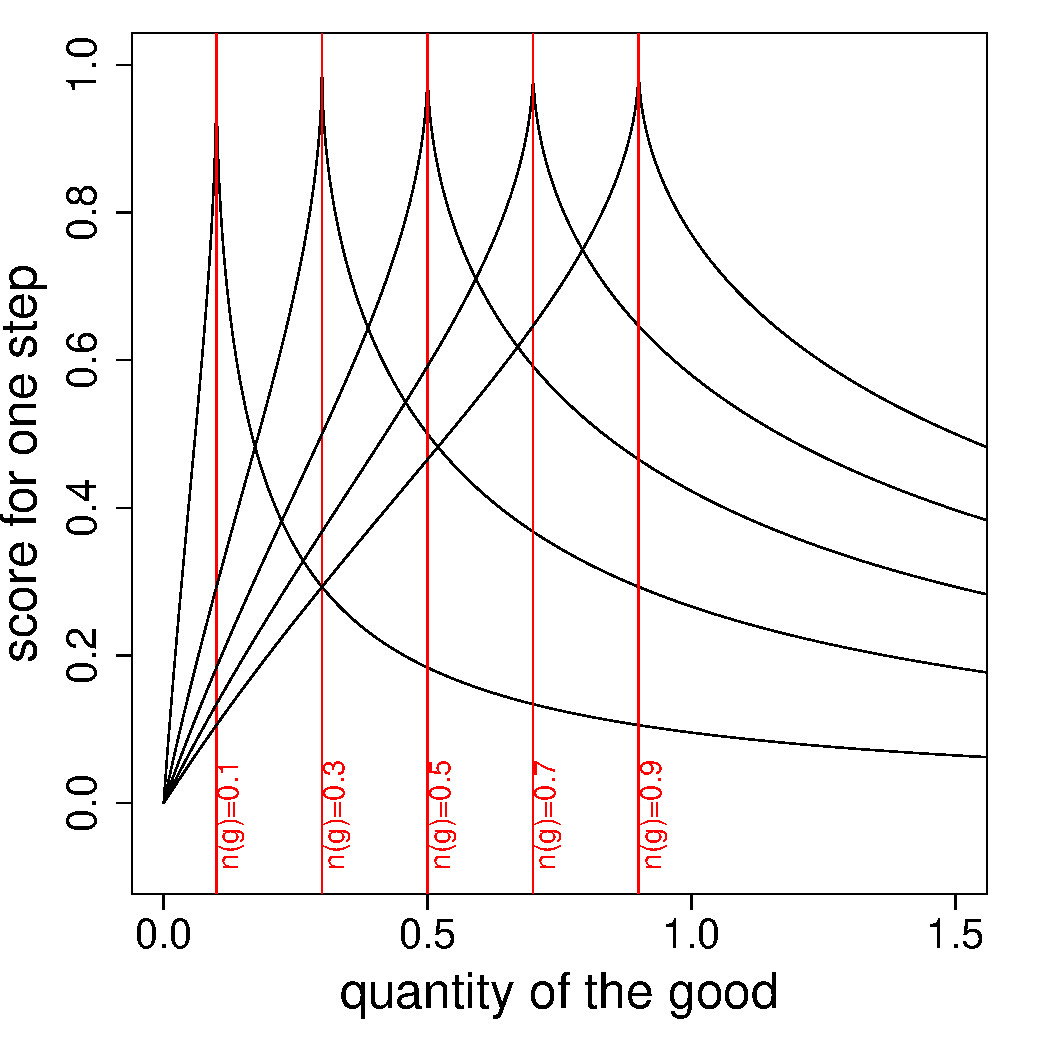
\includegraphics[width=.6\textwidth]{fitness.pdf}
		\end{center}
		\caption{The utility for different value in the ``universal scale''}
		\label{fig:fit}
	\end{figure}

\end{frame}
\end{document}




